\section{Analysis}

\subsection{Problem formulation}
As covered by Bilimoria the equations of motion for the rotation around principal axes of inertia are:
\begin{align}
I_x \dot{\Omega}_x + (I_z-I_y) \Omega_z \Omega_y &= \tau_x \\
I_y \dot{\Omega}_y + (I_x-I_z) \Omega_x \Omega_z &= \tau_y \\
I_z \dot{\Omega}_z + (I_y-I_x) \Omega_y \Omega_x &= \tau_z 
\end{align}

For simplicity, we will assume that the vehicle is symmetric and therefore all three moments of inertia are identical and equal to $I$. Figure Under those conditions the equations of motion decouple into:
\begin{align}
I \dot{\Omega}_x &= \tau_x \\
I \dot{\Omega}_y &= \tau_y \\
I \dot{\Omega}_z &= \tau_z 
\end{align}

Figure \ref{fig:symmetricBody} offers a depiction of such a system. The equations of motion above can be expressed in vector notation in a more compact manner:
\begin{equation}
I \vec{\Omega} = \vec{\tau}
\end{equation}

\begin{figure}[h]
	\centering
	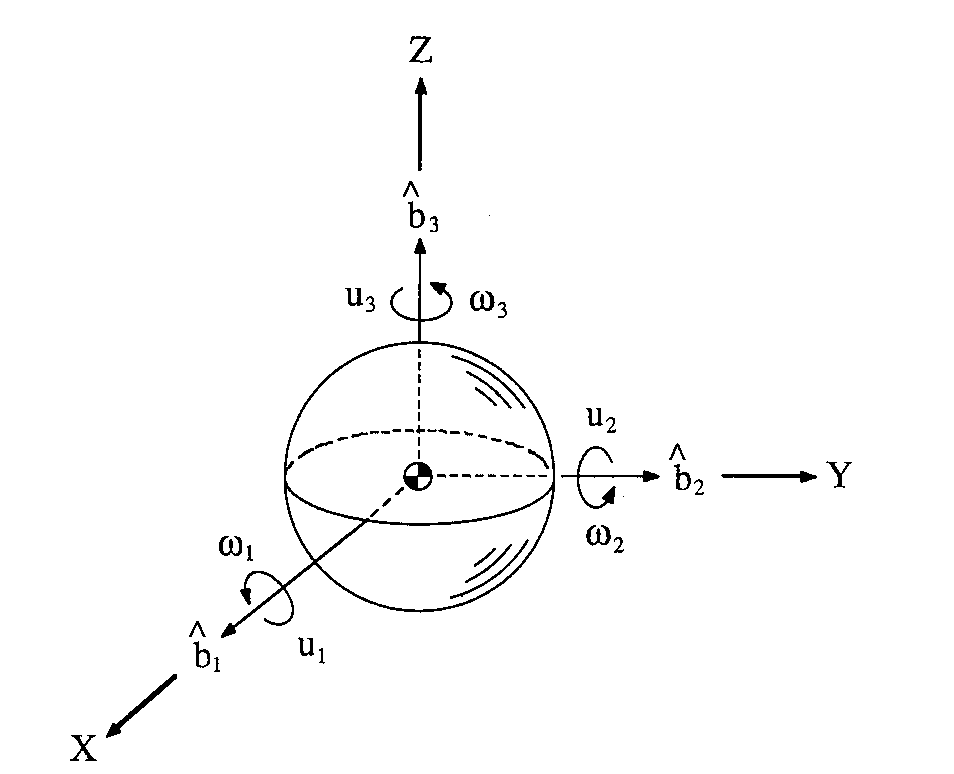
\includegraphics[height=6cm,keepaspectratio]{media/BilimoriaSymmetricBodyModel.png}
	\caption{Symmetric Body with controls along three axes. Original Source: Bilimoria \cite{bilimoria1993time}}
	\label{fig:symmetricBody}
\end{figure}

And the control is bounded by:
\begin{equation}
|\tau_x|^q + |\tau_y|^q + |\tau_z|^q \leq \tau_{max}^q
\end{equation}

Where $q$ is the norm of interest; this is a general way of bounding the control.  The most interesting norms will be the 2-norm and the infinity-norm ($\infty$-norm) corresponding to the maximum applied torque being independent of the direction, and to three independently bounded controls by $\tau_{max}$ respectively.

We can consider all three controls to be equally bounded by $\tau_{max}$ we can non-dimensionalize the equations of motion using $u_i = \tau_i / \tau_{max}$ and a characteristic time $t=\sqrt{I / \tau_{max}}$ so the characteristic angular velocity $\omega_i = \Omega_i \sqrt{I / \tau_{max}}$. The vector equation of motion now simplifies to its final form:
\begin{equation}
\label{omegadot}
\vec{\omega} = \vec{u}
\end{equation}

Beside the equations relating velocity to the control torques we need the equations of motion for the attitude quaternions. A description on how quaternions relate to euler angles and angular velocities can be found in Parwana and Kothari\cite{parwana2017quaternion} and useful relations for quaternion derivatives are provided by Graf \cite{graf2008quaternions}. For more details on the quaternion convention, or the derivation and partial differentiation we refer to the Appendix A. Our attitude quaternion is $q$ and we introduce an angular velocity quaternion $\omega = [0 \quad \vec{\omega}]^T$
\begin{equation}
\label{qdot}
\dot{q} = 1/2  \ q \circ \omega
\end{equation}

Now we are ready to state our optimization problem. Our performance index is the final time, which we will minimize, in other words:
\begin{equation}
\min J = t_f
\end{equation}
Subject to the vector process equations\ref{omegadot} and  \ref{qdot}. Our control, by the definition of the non-dimensionalization, is subject to $|u_i| \leq 1$. The initial and final states are fixed and defined by the maneuver to be optimized:
\begin{align}
 q(0) &= \left[ 1 \quad 0 \quad 0 \quad 0 \right]^T \\
 q(t_f) &= q_f \\
 \vec{\omega}(0) &= \vec{\omega}(t_f) = 0
\end{align}

The only free boundary is the final time $t_f$ which is the performance index to be minimized.

\subsection{Hamiltonian and co-state equations}
With the formulation for the equations of motion we define the Hamiltonian for the motion:
\begin{equation}
H(x,u,\lambda) = \frac{1}{2} \lambda_q^T (q \circ \omega) + \lambda_\omega^T \vec{u}
\end{equation}

Where $\lambda_q$ and $\lambda_\omega$ are the co-state vectors with a size of 4 elements and 3 elements respectively. We realize that, since there is no explicit time dependence, the Hamiltonian is constant throughout the motion. 

In order to get the co-state equations we get apply the Euler-Lagrange equations and find the appropriate derivatives. In order to simplify the resulting expressions Matrix calculus is used to come up with more compact expressions, see Appendix A for details on the derivation. The expression for the attitude co-states is:
\begin{equation}
\label{lambdaqDot}
\dot{\lambda}_q = - \frac{\partial H}{\partial q} =  \frac{1}{2} \lambda_q \circ \omega
\end{equation}

The partial derivative for $\dot{\lambda}_\omega$ depends on omega which appears only in the quaternion product, but it cannot be obtained straight forward using the expressions for quaternion derivatives since $\dot{\lambda}_\omega$ is not a 4 element vector. However, if we extend it to a 4 element vector where the first element is forced to be 0, we can find the partial derivative in terms of the imaginary part of the quaternion derivative.
\begin{equation}
\dot{\lambda}_\omega = - \frac{\partial H}{\partial \omega} = - \frac{1}{2} \text{Im}(q' \circ \lambda_q)
\end{equation}

We now look at the boundary conditions. In the problem statement we have stated that the final and initial states are fixed, also the initial time is fixed. Since the only free state is the final time $t_f$ we look for the associated condition in the transversality condition:
\begin{equation}
  H_f dt_f - \lambda^T dx_f + dg = H_f dt_f - \lambda^T dx_f + dt_f = (H_f + 1) dt_f \implies H_f + 1 = 0
\end{equation}

Also, since the Hamiltonian is constant we have that throughout the motion:
\begin{equation}
 H = -1
\end{equation}

\subsection{Derivation of the optimal control}
The control logic is that of a bang-bang controller, which can be expected for a minimum-time type strategy with some modifications. Because of this, we have the possibility of having singular sub-arcs. Later we will have to study the possible consequences on the control.

In order to find the optimal control we recognize that we have an inequality constraint in the control of the following form:
\begin{equation}
1 =  |u_x|^q + |u_y|^q + |u_z|^q
\end{equation}
This means that $H_u^*=0$ cannot be directly satisfied. This bound on the control does is not a switching function neither, so we have to apply Pontryagin's Minimum Principle in its most basic form. We have to look for the optimal control such that:
\begin{equation}
H(x^*, u^*, \lambda^*) \leq H(X^*, u, \lambda^*)
\end{equation}

Or equivalently for our Hamiltonian:
\begin{equation}
\lambda_\omega^{*T} \vec{u}^* \leq \lambda_\omega^{*T} \vec{u}
\end{equation}

Since the expression above is linear in terms of $\vec{u}$ the minimum will necessarily lie on the inequality constraint of the norm of $\vec{u}$. We introduce the constraint in the expression above by solving for $u_z$ in terms of $u_x$ and $u_y$ and the sign of $u_z$ which we don't know yet:
\begin{equation}
\label{uzFromNorm}
u_z = \text{sgn}(u_z) \ (1 - |u_x|^q - |u_y|^q)^{\frac{1}{q}}
\end{equation}

Now we have to look for a minimum of:
\begin{equation}
\label{unconstrainedOptimalControl}
\mathcal{L} = \lambda_{\omega_x} u_x + \lambda_{\omega_y} u_y + \text{sgn}(u_z) \lambda_{\omega_3} (1 - |u_x|^q - |u_y|^q)^{\frac{1}{q}}
\end{equation}

In order to find the minimum we take partial derivatives with respect $u_x$ and $u_y$. In the derivatives we identify the expression for $|u_z|$ so we substitute it back: 
\begin{align}
\label{partialLx}
\frac{\partial \mathcal{L}}{\partial u_x} &= 0 =\lambda_{\omega_x} - \text{sgn}(u_x u_z) \ \lambda_{\omega_z} \ (1 - |u_x|^q - |u_y|^q)^{\frac{1-q}{q}} |u_x|^{q-1} = \lambda_{\omega_x} - \text{sgn}(u_x u_z) \ \lambda_{\omega_z} \ |u_z|^{1-q} |u_x|^{q-1}\\
\label{partialLy}
\frac{\partial \mathcal{L}}{\partial u_y} &= 0 = \lambda_{\omega_y} - \text{sgn}(u_y u_z) \ \lambda_{\omega_z} \ (1 - |u_x|^q - |u_y|^q)^{\frac{1-q}{q}} |u_y|^{q-1} = \lambda_{\omega_y} - \text{sgn}(u_y u_z) \ \lambda_{\omega_z} \ |u_z|^{1-q} |u_y|^{q-1}
\end{align}

And on the expressions above we solve for $u_x$ or $u_y$:
\begin{align}
&\lambda_{\omega_{x,y}} - \text{sgn}(u_{x,y} u_z) \ \lambda_{\omega_z} \ |u_z|^{1-q} |u_{x,y}|^{q-1} = 0 \\
\implies &
\text{sgn}(u_{x,y}) |u_{x,y}|^{q-1} = \frac{\lambda_{\omega_{x,y}}}{\lambda_{\omega_z}} \text{sgn}(u_z) \ |u_z|^{q-1} \\
\implies &
\text{sgn}(u_{x,y}) |u_{x,y}| = \text{sgn}\left(\frac{\lambda_{\omega_{x,y}}}{\lambda_{\omega_z}}\right) \left|\frac{\lambda_{\omega_{x,y}}}{\lambda_{\omega_z}}\right|^{\frac{1}{q-1}}
 \text{sgn}(u_z) \ |u_z| \\
= &
\label{uxyFromuz}
u_{x,y} = \text{sgn}\left(\frac{\lambda_{\omega_{x,y}}}{\lambda_{\omega_z}}\right) \left|\frac{\lambda_{\omega_{x,y}}}{\lambda_{\omega_z}}\right|^{\frac{1}{q-1}}
u_z
\end{align}

And substituting these expressions in the expression we obtained in \ref{uzFromNorm} we obtain:
\begin{align}
& |u_z| = 
\left(
\frac{|u_z|^q}{|u_z|^q} \left|\frac{\lambda_{\omega_{z}}}{\lambda_{\omega_z}}\right|^{\frac{q}{q-1}}
|u_z|^q- \left|\frac{\lambda_{\omega_{x}}}{\lambda_{\omega_z}}\right|^{\frac{q}{q-1}}
|u_z|^q - \left|\frac{\lambda_{\omega_{x}}}{\lambda_{\omega_z}}\right|^{\frac{q}{q-1}}
|u_z|^q
\right)^{\frac{1}{q}} \\
\implies & 
|\lambda_{\omega_z}|^{\frac{q}{q-1}} = 
\frac{1}{|u_z|^q} |\lambda_{\omega_{z}}|^{\frac{q}{q-1}}
- |\lambda_{\omega_{x}}|^{\frac{q}{q-1}}
- |\lambda_{\omega_{x}}|^{\frac{q}{q-1}}
\\ \implies &
\frac{1}{|\lambda_{\omega_{z}}|^{\frac{q}{q-1}}}
|\lambda_{\omega_z}|^{\frac{q}{q-1}} + |\lambda_{\omega_{x}}|^{\frac{q}{q-1}}
+ |\lambda_{\omega_{x}}|^{\frac{q}{q-1}} = 
\frac{1}{|u_z|^q}
\\ \implies &
|u_z| = 
\frac{|\lambda_{\omega_{z}}|^{\frac{1}{q-1}}}
{\left[ |\lambda_{\omega_x}|^{\frac{q}{q-1}} + |\lambda_{\omega_y}|^{\frac{q}{q-1}} + |\lambda_{\omega_z}|^{\frac{q}{q-1}}\right]^\frac{1}{q}}
\end{align}

These last expressions define the magnitude of each control input as function of the magnitude of the co-states, but we still don't know how to find the sign of $u_z$. However to pick the right sign we just need to recall that our goal is to minimize the Hamiltonian, therefore we have to pick the sign with the opposite sign to $\lambda_{\omega_z}$. 

%% Legendre-Clebsch condition approach
\iffalse
In order to find it we make use of the Legendre-Clebsch condition on the unconstrained version of the problem we found on \ref{unconstrainedOptimalControl}. In \ref{partialLx}, \ref{partialLy} we found the first derivatives, in order to verify the Legendre-condition we take the second derivatives:
\begin{align}
\frac{\partial^2 \mathcal{L}}{{\partial u_x}^2} &=
-\text{sgn}(u_z) \ \lambda_{\omega_z} \ \left( -(1 - |u_x|^q - |u_y|^q)^{\frac{1-2q}{q}} |u_x|^{2q-2} + \ (1 - |u_x|^q - |u_y|^q)^{\frac{1-q}{q}} |u_x|^{q-2} \right) \\
&= -\text{sgn}(u_z) \ \lambda_{\omega_z} \ \left(-|u_z|^{1-2q} |u_x|^{2q-2} + |u_z|^{1-q} |u_x|^{q-2} \right) \nonumber
\\
\frac{\partial^2 \mathcal{L}}{{\partial u_y}^2} &= 
-\text{sgn}(u_z) \ \lambda_{\omega_z} \ \left( -(1 - |u_x|^q - |u_y|^q)^{\frac{1-2q}{q}} |u_y|^{2q-2} + \ (1 - |u_x|^q - |u_y|^q)^{\frac{1-q}{q}} |u_y|^{q-2} \right) \\
&= -\text{sgn}(u_z) \ \lambda_{\omega_z} \ \left(-|u_z|^{1-2q} |u_y|^{2q-2} + |u_z|^{1-q} |u_y|^{q-2} \right) \nonumber
\\
\frac{\partial^2 \mathcal{L}}{{\partial u_y}^2} &= 
\text{sgn}(u_z u_x u_y) \ \lambda_{\omega_z} \ \left( (1 - |u_x|^q - |u_y|^q)^{\frac{1-2q}{q}} |u_y|^{q-1} |u_x|^{q-1} \right) \\
&= \text{sgn}(u_z u_x u_y) \ \lambda_{\omega_z} \ |u_z|^{1-2q} |u_y|^{q-1} |u_x|^{q-1}
\end{align}
\fi

Once we have found the right $u_z$ we can solve for $u_{x,y}$, using \ref{uxyFromuz}. The expression for all three controls becomes similar, as it could be expected:
\begin{equation}
\label{lqControl}
u_i = 
\frac{-\text{sgn}(\lambda_{\omega_{i}}) |\lambda_{\omega_{i}}|^{\frac{1}{q-1}}}
{\left[ |\lambda_{\omega_x}|^{\frac{q}{q-1}} + |\lambda_{\omega_y}|^{\frac{q}{q-1}} + |\lambda_{\omega_z}|^{\frac{q}{q-1}}\right]^\frac{1}{q}}
\end{equation}

Finally, we have to consider the possibility of singular control. In order to rule it out, we recall the $H=-1$ condition obtained from the transversality condition. This allows us to guarantee that there will be non singular sub-arcs. Singular subarcs will only happen if $\lambda_\omega = 0$ for a finite interval, this implies that $\dot{\lambda}_\omega = 0$, but since $q$ is an atittude quaternion, $\dot{\lambda}_\omega = 0$ will only happen if $\lambda_q=0$. This cannot happen at the same time that $\lambda_\omega = 0$ since that would make the Hamiltonian vanish, contradicting the transversality condition. Since there are no singular sub-arcs the controller above satisfies the necessary conditions for an optimal control. 

The controller structure is fundamentally of a bang-bang nature as anticipated. There is a component controlling the amplitude of the control to the different actuators, but on top of this amplitude allocation, the sign is controlled in the same fashion as a usual bang-bang control. Choosing a norm will determine the behavior of the control amplitude allocation, allowing for more independence between the controls that will lead to more and more complex control profiles and possible faster maneuvers since the set of possible controls increases with the norm. 

In the limit, where the norm goes to infinity the controls become completely independent with the form of switching functions. Each control component must satisfy $|u_i|\leq 1$. Then from the limit of the control in \ref{lqControl}, or following the usual reasoning for switching functions minimizing the Hamiltonian we get:
\begin{equation}
\label{lInfinityControl}
u_i = -\text{sgn}(\lambda_{\omega_{i}})
\end{equation}